\documentclass[14pt]{extbook}
\usepackage{multicol, enumerate, enumitem, hyperref, color, soul, setspace, parskip, fancyhdr} %General Packages
\usepackage{amssymb, amsthm, amsmath, latexsym, units, mathtools} %Math Packages
\everymath{\displaystyle} %All math in Display Style
% Packages with additional options
\usepackage[headsep=0.5cm,headheight=12pt, left=1 in,right= 1 in,top= 1 in,bottom= 1 in]{geometry}
\usepackage[usenames,dvipsnames]{xcolor}
\usepackage{dashrule}  % Package to use the command below to create lines between items
\newcommand{\litem}[1]{\item#1\hspace*{-1cm}\rule{\textwidth}{0.4pt}}
\pagestyle{fancy}
\lhead{Progress Quiz 7}
\chead{}
\rhead{Version C}
\lfoot{4173-5738}
\cfoot{}
\rfoot{Spring 2021}
\begin{document}

\begin{enumerate}
\litem{
Choose the equation of the function graphed below.
\begin{center}
    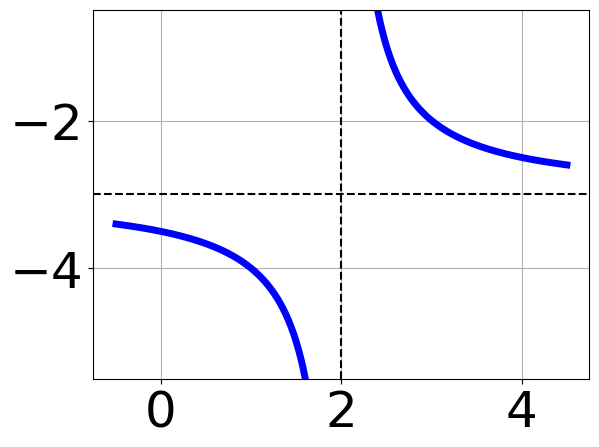
\includegraphics[width=0.5\textwidth]{../Figures/rationalGraphToEquationC.png}
\end{center}
\begin{enumerate}[label=\Alph*.]
\item \( f(x) = \frac{1}{x - 2} - 3 \)
\item \( f(x) = \frac{-1}{(x + 2)^2} - 3 \)
\item \( f(x) = \frac{-1}{x + 2} - 3 \)
\item \( f(x) = \frac{1}{(x - 2)^2} - 3 \)
\item \( \text{None of the above} \)

\end{enumerate} }
\litem{
Determine the domain of the function below.\[ f(x) = \frac{6}{24x^{2} -60 x + 36} \]\begin{enumerate}[label=\Alph*.]
\item \( \text{All Real numbers except } x = a, \text{ where } a \in [0.5, 1.3] \)
\item \( \text{All Real numbers except } x = a \text{ and } x = b, \text{ where } a \in [0.5, 1.3] \text{ and } b \in [1.2, 1.6] \)
\item \( \text{All Real numbers except } x = a, \text{ where } a \in [23, 24.6] \)
\item \( \text{All Real numbers.} \)
\item \( \text{All Real numbers except } x = a \text{ and } x = b, \text{ where } a \in [23, 24.6] \text{ and } b \in [35.8, 37.4] \)

\end{enumerate} }
\litem{
Solve the rational equation below. Then, choose the interval(s) that the solution(s) belongs to.\[ \frac{7x}{3x -6} + \frac{-7x^{2}}{18x^{2} -57 x + 42} = \frac{-7}{6x -7} \]\begin{enumerate}[label=\Alph*.]
\item \( x_1 \in [-0.92, -0.74] \text{ and } x_2 \in [1.01,1.73] \)
\item \( \text{All solutions lead to invalid or complex values in the equation.} \)
\item \( x \in [0.61,1.18] \)
\item \( x \in [1.39,1.65] \)
\item \( x_1 \in [-0.92, -0.74] \text{ and } x_2 \in [1.81,2.66] \)

\end{enumerate} }
\litem{
Determine the domain of the function below.\[ f(x) = \frac{4}{9x^{2} +33 x + 30} \]\begin{enumerate}[label=\Alph*.]
\item \( \text{All Real numbers except } x = a \text{ and } x = b, \text{ where } a \in [-18.56, -17.7] \text{ and } b \in [-15.63, -14.7] \)
\item \( \text{All Real numbers except } x = a \text{ and } x = b, \text{ where } a \in [-2.39, -2] \text{ and } b \in [-1.67, -1.5] \)
\item \( \text{All Real numbers except } x = a, \text{ where } a \in [-2.39, -2] \)
\item \( \text{All Real numbers.} \)
\item \( \text{All Real numbers except } x = a, \text{ where } a \in [-18.56, -17.7] \)

\end{enumerate} }
\litem{
Choose the graph of the equation below.\[ f(x) = \frac{1}{x - 2} - 3 \]\begin{enumerate}[label=\Alph*.]
\begin{multicols}{2}\item 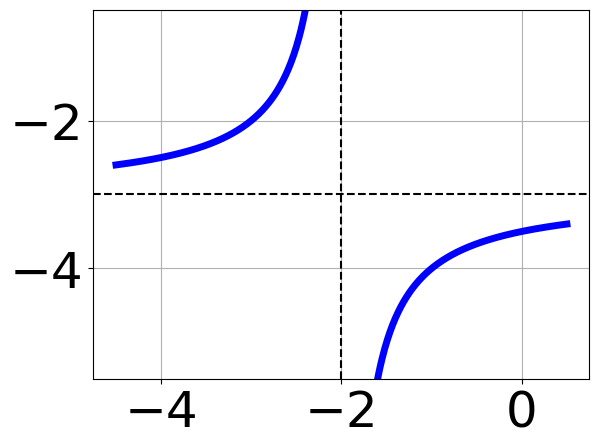
\includegraphics[width = 0.3\textwidth]{../Figures/rationalEquationToGraphAC.png}\item 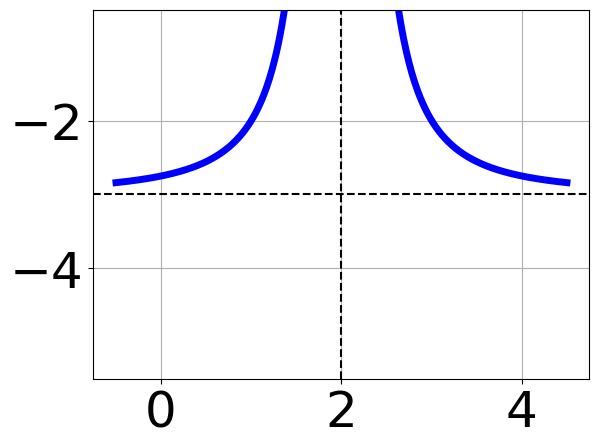
\includegraphics[width = 0.3\textwidth]{../Figures/rationalEquationToGraphBC.png}\item 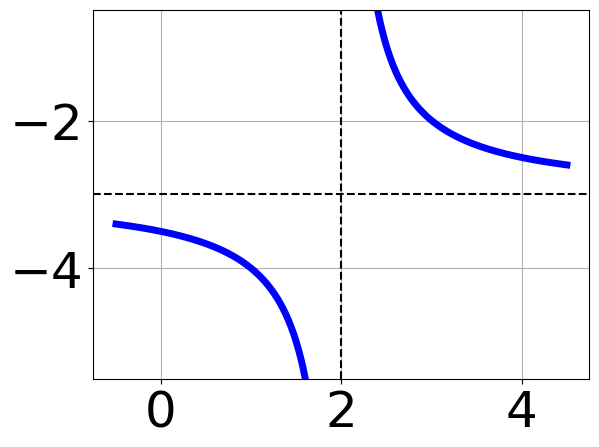
\includegraphics[width = 0.3\textwidth]{../Figures/rationalEquationToGraphCC.png}\item 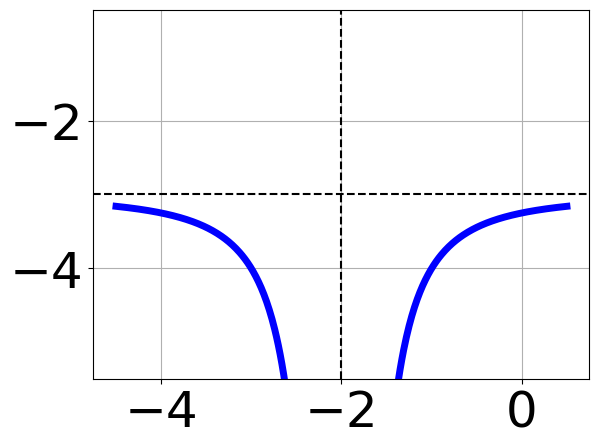
\includegraphics[width = 0.3\textwidth]{../Figures/rationalEquationToGraphDC.png}\end{multicols}\item None of the above.
\end{enumerate} }
\litem{
Choose the equation of the function graphed below.
\begin{center}
    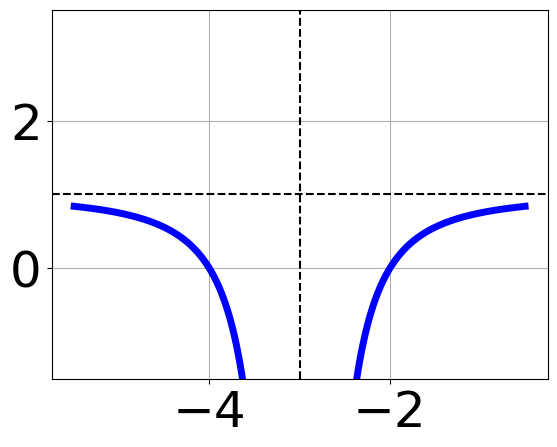
\includegraphics[width=0.5\textwidth]{../Figures/rationalGraphToEquationCopyC.png}
\end{center}
\begin{enumerate}[label=\Alph*.]
\item \( f(x) = \frac{1}{x - 3} + 1 \)
\item \( f(x) = \frac{-1}{x + 3} + 1 \)
\item \( f(x) = \frac{1}{(x - 3)^2} + 1 \)
\item \( f(x) = \frac{-1}{(x + 3)^2} + 1 \)
\item \( \text{None of the above} \)

\end{enumerate} }
\litem{
Choose the graph of the equation below.\[ f(x) = \frac{-1}{x - 3} - 2 \]\begin{enumerate}[label=\Alph*.]
\begin{multicols}{2}\item 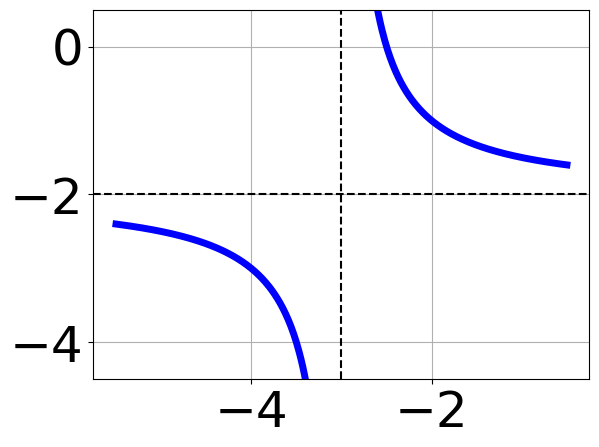
\includegraphics[width = 0.3\textwidth]{../Figures/rationalEquationToGraphCopyAC.png}\item 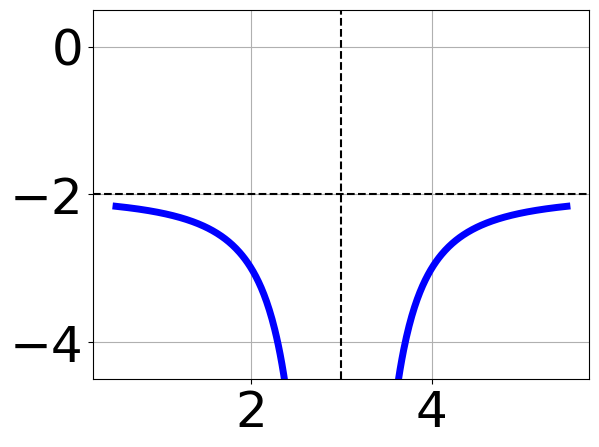
\includegraphics[width = 0.3\textwidth]{../Figures/rationalEquationToGraphCopyBC.png}\item 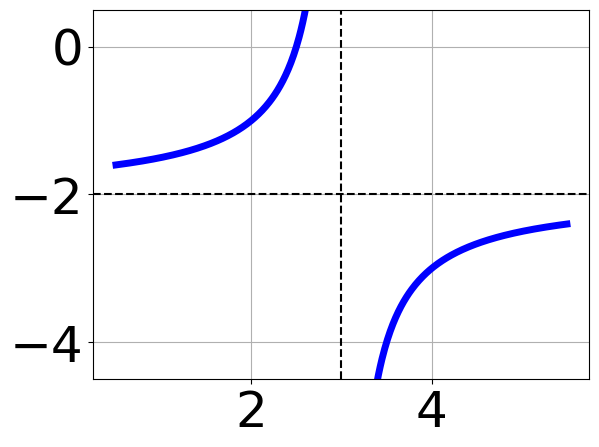
\includegraphics[width = 0.3\textwidth]{../Figures/rationalEquationToGraphCopyCC.png}\item 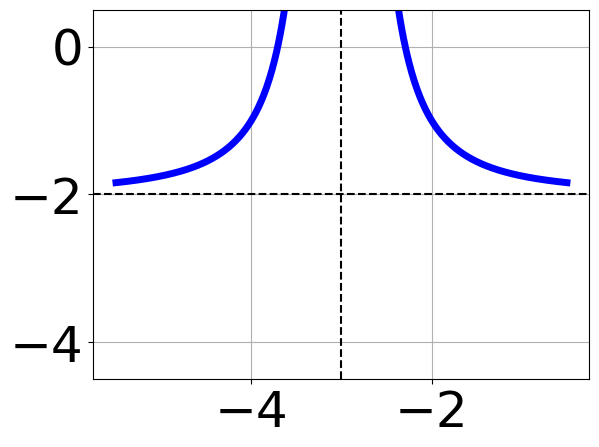
\includegraphics[width = 0.3\textwidth]{../Figures/rationalEquationToGraphCopyDC.png}\end{multicols}\item None of the above.
\end{enumerate} }
\litem{
Solve the rational equation below. Then, choose the interval(s) that the solution(s) belongs to.\[ \frac{7}{8x -6} + -7 = \frac{-6}{48x -36} \]\begin{enumerate}[label=\Alph*.]
\item \( x \in [0.89,1.89] \)
\item \( \text{All solutions lead to invalid or complex values in the equation.} \)
\item \( x \in [-0.61,0.39] \)
\item \( x_1 \in [-0.11, 2.89] \text{ and } x_2 \in [0.94,1.02] \)
\item \( x_1 \in [-0.61, 0.39] \text{ and } x_2 \in [0.77,0.94] \)

\end{enumerate} }
\litem{
Solve the rational equation below. Then, choose the interval(s) that the solution(s) belongs to.\[ \frac{6x}{2x -3} + \frac{-7x^{2}}{-10x^{2} +27 x -18} = \frac{5}{-5x + 6} \]\begin{enumerate}[label=\Alph*.]
\item \( \text{All solutions lead to invalid or complex values in the equation.} \)
\item \( x_1 \in [-0.42, -0.15] \text{ and } x_2 \in [1.32,1.56] \)
\item \( x_1 \in [-0.42, -0.15] \text{ and } x_2 \in [1.01,1.22] \)
\item \( x \in [1.2,1.47] \)
\item \( x \in [1,1.1] \)

\end{enumerate} }
\litem{
Solve the rational equation below. Then, choose the interval(s) that the solution(s) belongs to.\[ \frac{25}{45x + 45} + 1 = \frac{25}{45x + 45} \]\begin{enumerate}[label=\Alph*.]
\item \( x_1 \in [-3, 0] \text{ and } x_2 \in [0.8,1.4] \)
\item \( \text{All solutions lead to invalid or complex values in the equation.} \)
\item \( x_1 \in [-3, 0] \text{ and } x_2 \in [-1.6,-0.6] \)
\item \( x \in [0,2] \)
\item \( x \in [-1.0,1.0] \)

\end{enumerate} }
\end{enumerate}

\end{document}